\documentclass[12pt]{article}
\usepackage[top=1in, bottom=1in, left=1in, right=1in]{geometry}

\usepackage{setspace}
\onehalfspacing

\usepackage{amssymb}
%% The amsthm package provides extended theorem environments
\usepackage{amsthm}
\usepackage{epsfig}
\usepackage{times}
\renewcommand{\ttdefault}{cmtt}
\usepackage{amsmath}
\usepackage{graphicx} % for graphics files
\usepackage{tabu}

% Draw figures yourself
\usepackage{tikz} 

% writing elements
\usepackage{mhchem}

\usepackage{paralist}

% The float package HAS to load before hyperref
\usepackage{float} % for psuedocode formatting
\usepackage{xspace}

% from Denovo Methods Manual
\usepackage{mathrsfs}
\usepackage[mathcal]{euscript}
\usepackage{color}
\usepackage{array}
\usepackage{bm}

\usepackage[parfill]{parskip}

% math syntax
\newcommand{\SN}{S$_N$}
\newcommand{\vd}{\bm{\cdot}} % slightly bold vector dot
\newcommand{\grad}{\vec{\nabla}} % gradient
\newcommand{\ud}{\mathop{}\!\mathrm{d}} % upright derivative symbol
\def\bal#1\nal{\begin{align}#1\end{align}}
\def\bala#1\nala{\begin{align*}#1\end{align*}}
\newcommand{\f}{\frac}
\newcommand{\ux}{\ensuremath{\vec{r}}}
\newcommand{\un}{{\bm n}}
\newcommand{\unab}{{\bf \nabla}}
\newcommand{\ep}{\varepsilon}
\newcommand{\uom}{\ensuremath{\hat{\Omega}}}
  \newcommand{\bl}{\big<}
  \newcommand{\bg}{\big>}
    \newcommand{\n}{ \noindent}



\newcommand{\nth}{n\ensuremath{^{\text{th}}} }
\newcommand{\ve}[1]{\ensuremath{\mathbf{#1}}}
\newcommand{\Macro}{\ensuremath{\Sigma}}
\newcommand{\rvec}{\ensuremath{\vec{r}}}
\newcommand{\vecr}{\ensuremath{\vec{r}}}
\newcommand{\omvec}{\ensuremath{\hat{\Omega}}}
\newcommand{\vOmega}{\ensuremath{\hat{\Omega}}}
\newcommand{\even}{\ensuremath{\phi^g}}
\newcommand{\odd}{\ensuremath{\vartheta^g}}
\newcommand{\evenp}{\ensuremath{\phi^{g'}}}
\newcommand{\oddp}{\ensuremath{\vartheta^{g'}}}
\newcommand{\Sn}{\ensuremath{S_N} }
\newcommand{\Ye}[2]{\ensuremath{Y^e_{#1}(\vOmega_#2)}}
\newcommand{\sigg}[1]{\ensuremath{\Macro^{gg'}_{s\,#1}}}
\newcommand{\psig}{\ensuremath{\psi^g}}
%---------------------------------------------------------------------------
%---------------------------------------------------------------------------
\begin{document}
\begin{center}
{\bf NE 255, Fa16 \\
Transport in Stochastic Mixtures\\
November 29, 2016}
\end{center}

\setlength{\unitlength}{1in}
\begin{picture}(6,.1) 
\put(0,0) {\line(1,0){6.25}}         
\end{picture}

These notes are derived from the course ``Advanced Topics in Transport Theory'', taught at RWTH Aachen University, Germany, on the Summer of 2013. 

\section*{The Atomic Mix Model (empirical motivation)}

Let us consider the integro-differential transport equation.
In a deterministic medium, the total cross section $\Sigma_t$, the scattering kernel $\Sigma_s$, and the source $Q$ are known prescribed functions of their arguments.
Thus, in order to find an expression for the angular flux $\psi$, one must solve this equation subject to the boundary and initial conditions. 

Now we consider neutron transport in a heterogeneous volume $V$ such that the boundary $\partial V$ of $V$ is specified, but the interior structure of $V$ is not.
Specifically, we restrict our attention to the case in which $V$ consists of two random immiscible materials denoted by an index $i$, with $i=1,2$.
We can imagine $V$ as a heterogeneous volume consisting of randomly distributed chunks of random sizes and shapes of material 1 imbedded in material 2.
If we consider a particle traversing the mixture along a random path, it will pass through alternating segments of these two materials, as we can see in Figure \ref{fig_trav_chunks}.
\begin{figure}[h]
\centering
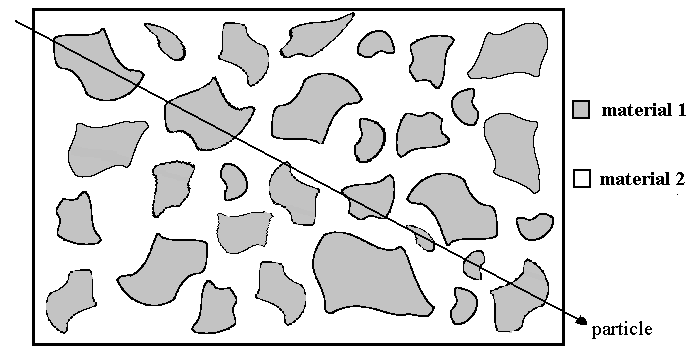
\includegraphics[height=6.45 cm,width= 12.9 cm]{traversing_chunks}
%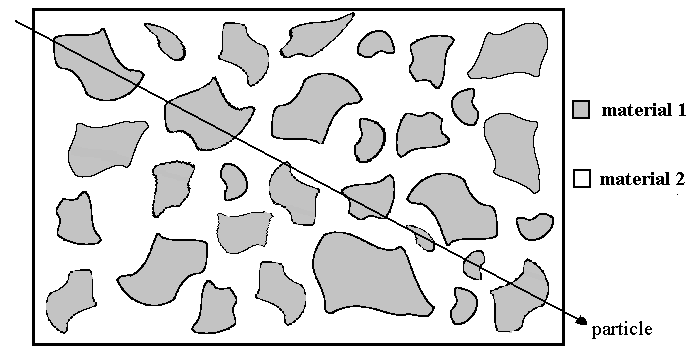
\includegraphics[height=6.45 cm,width= 12.9 cm]{traversing_chunks.jpg}
\caption{\footnotesize{Particle traversing the mixture along a random path}}\label{fig_trav_chunks}
\end{figure}

The quantities $\Sigma_t$, $\Sigma_s$, and $Q$ are considered as discrete random variables.
That is, in the $i$th material these elements are denoted by $\Sigma_{ti}(\bm x,E,t)$, $\Sigma_{si}(\bm x,E'\rightarrow E,\bm\Omega'\cdot\bm\Omega,t)$, and $Q_i(\bm x,E,\bm\Omega,t)$.
The stochasticity of the problem is that we have only a probabilistic idea about which material occupies the space point $\bm x$ at a time $t$.
Therefore, since we are considering $\Sigma_t$, $\Sigma_s$, and $Q$ as random variables, we must also consider the angular flux $\psi$ as a random variable.
We want to find an expression for $\bl\psi\bg$, the ensemble-averaged angular flux (expected value) of $\psi$.

For convenience, let us consider the case of transport in a non-scattering (i.e. purely absorbing) medium.
Thinking about $\bm\Omega\cdot\nabla$ as a directional derivative, we can rewrite the time-dependent transport equation as
\begin{equation}\label{nonscatdirec}
\frac{1}{v}\frac{\partial\psi(u,t)}{\partial t}+\frac{\partial\psi(u,t)}{\partial u}+
\Sigma_t(u,t)\psi(u,t)=Q(u,t),
\end{equation}
\n where $u$ denotes the spatial variable in the direction $\bm\Omega$.
One must notice that $\textrm{Eq.}\ ($\ref{nonscatdirec}) describes particle transport at each energy $E$ and direction $\bm\Omega$, which are omitted since they are only parameters.
We let $\bl W \bg$ denote the ensemble average of any random variable $W$, and define $\tilde W$ as the deviation of $W$ from $\bl W \bg$.
Then $\bl \tilde W \bg = 0$, and $W = \bl W\bg + \tilde W$.
Using this notation we ensemble-average $\textrm{Eq.}\ ($\ref{nonscatdirec}) to obtain
\begin{equation}\label{nonscataverage}
\frac{1}{v}\frac{\partial\bl\psi\bg}{\partial t}+\frac{\partial\bl\psi\bg}{\partial u}+
\bl\Sigma_t\bg\bl\psi\bg + \bl \tilde \Sigma_t \tilde \psi\bg = \bl Q\bg.
\end{equation}
The values of $\bl\Sigma_t\bg$ and $\bl Q\bg$ in this equation are defined in terms of the properties of materials 1 and 2.
Defining $p_i(u,t)$ as the probability of presence of the material $i$ at position $u$ at time $t$, then 
\begin{equation}
p_1(u,t)+p_2(u,t) = 1,
\end{equation}
\n and we can write 
\begin{equation}
\bl \Sigma_t(u,t)\bg = p_1(u,t)\Sigma_{t1}(u,t)+p_2(u,t)\Sigma_{t2}(u,t),
\end{equation}
\begin{equation}
\bl Q(u,t)\bg = p_1(u,t)Q_1(u,t)+p_2(u,t)Q_2(u,t).
\end{equation}

If we write the characteristic chord length (mean chord length) for the chunks of material $i$ as $\Lambda_i$ and assume that
\begin{equation}\label{chord}
\Sigma_{ti}\Lambda_i \ll 1, \hspace{0.5 cm} i=1,2,
\end{equation}
then a particle between collisions is likely to travel a distance that spans many chunks of materials 1 and 2.
This means that $\Lambda_i$ is very small when compared with the mean free path $\bl s\bg$.
On physical grounds, this assumption appropriately describes vanishingly small chunks in the mixture, which can be understood as if the two components of the system were mixed at the atomic level.

When $\textrm{Eq.}\ ($\ref{chord}) is satisfied, it is physically intuitive that the transport process will be well-approximated by the process that holds when the chunk
sizes are zero in the limit (the atomic mix limit).
Moreover, when the chunk sizes shrink, the deviations in the angular flux should also shrink, and $\tilde \psi$ will go to zero.
Hence, the 
cross correlation term $\bl \tilde \Sigma_t \tilde \psi\bg$ in $\textrm{Eq.}\ ($\ref{nonscataverage}) can be safely neglected, and $\textrm{Eq.}\ ($\ref{nonscataverage}) becomes 
\begin{equation}
\frac{1}{v}\frac{\partial\bl\psi\bg}{\partial t}+\frac{\partial\bl\psi\bg}{\partial u}+
\bl\Sigma_t\bg\bl\psi\bg = \bl Q\bg,
\end{equation}
\n which is closed for the ensemble-averaged angular flux $\bl\psi\bg$.
This equation represents the atomic mix description of $\textrm{Eq.}\ ($\ref{nonscatdirec}).

Applying the same arguments on the general form of the transport equation, the atomic mix description of stochastic transport, including scattering, is given by
\begin{equation}\label{atmixeqgeral}
\begin{split}
&\frac{1}{v}\frac{\partial \bl\psi(\bm x,E,\bm\Omega,t)\bg}{\partial t} + 
\bm\Omega\cdot \nabla  \bl\psi(\bm x,E,\bm\Omega,t)\bg +
 \bl\Sigma_t (\bm x,E,t)\bg\bl\psi(\bm x,E,\bm\Omega,t)\bg  = 
\\&\hspace{0.8 cm} =
\int_0^{\infty}\int_{4\pi}\bl\Sigma_s(\bm x, E'\rightarrow E,\bm\Omega'\cdot\bm\Omega,t)\bg
\bl\psi(\bm x,E',\bm\Omega',t)\bg d\Omega'dE'+\bl Q(\bm x, E, \bm\Omega,t)\bg  ,
\end{split}
\end{equation}
with 
\begin{equation}
\bl \psi(\bm x_s,E,\bm\Omega,t)\bg = \bl\psi_s(\bm x_s,E,\bm\Omega,t)\bg, \hspace{0.5 cm} \mathbf{n}\cdot\bm\Omega<0,
\end{equation}
\begin{equation}
\bl \psi(\bm x,E,\bm\Omega,0)\bg = \bl\psi_0(\bm x,E,\bm\Omega)\bg. 
\end{equation}
\n Here 
\begin{equation}\label{expected_value_general}
\bl W\bg = p_1(\bm x,t)W_1 + p_2(\bm x,t)W_2,
\end{equation}
\n where $W$ stands for $\Sigma_t$, $\Sigma_s$, and $Q$. 
The neglected cross correlation terms are $\bl\tilde\Sigma_t\tilde\psi\bg$ and $\bl\tilde\Sigma_s\tilde\psi\bg$.
 

\section*{The Multiscale Expansion Technique for Deriving Atomic Mix}

So far we have discussed only an empirical way to obtain the atomic mix equation.
Now, we will derive a simplified version of the atomic mix equationus ing the formal procedure of multiscale expansions, following the idea presented by
Dumas and Golse \cite{dumas_00}.
(For those interested, the cited paper contains a rigorous derivation of the method, proving that the atomic mix approximation is an asymptotic limit of the particle transport equation as the chunk widths of the materials limit to zero.)

Let us consider time independent transport in a 3-D volume in which heterogeneities occur along one spatial dimension ($x$) only.
Moreover, let this volume consist of binary walls placed perpendicularly to the $x$-axis.
A transverse intersection of this volume is represented by the multilayered slab in Figure \ref{fig_multilayered}, where $\Lambda_i$ is
\begin{figure}[h]
\centering
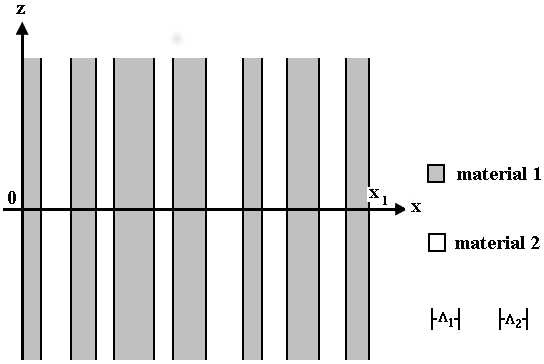
\includegraphics[height=6 cm,width= 9 cm]{multilayered}
%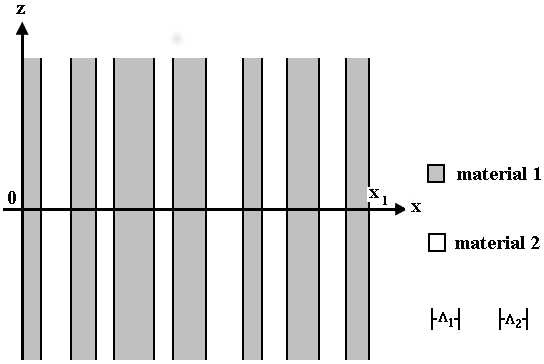
\includegraphics[height=6 cm,width= 9 cm]{multilayered.jpg}
\caption{\footnotesize{Multilayered slab - transverse volume intersection}}\label{fig_multilayered}
\end{figure}
the mean width of the regions of the homogeneous material $i$ ($i=1,2$).

Denoting the mean free path of a particle in this system as by $\bl s\bg$, we define
\begin{equation}
\Lambda = \frac{\Lambda_1+\Lambda_2}{2},
\end{equation}
and assuming that $\textrm{Eq.}\ ($\ref{chord}) holds, which characterizes a mixture at atomic level, we define the small parameter $\ep$ by 
\begin{equation}\label{defatmix}
\frac{\Lambda}{\bl s\bg} = \ep \ll 1.
\end{equation}

For simplicity, we will assume that the scattering process is both coherent and isotropic, and that the source $Q$ emmits particles isotropically.
It is therefore clear that $\Sigma_t$, $\Sigma_s$, and $Q$ will depend only upon the spatial variable $x$, since our assumptions allow us to consider energy $E$ as a simple parameter. 
In this case, the steady-state transport equation is given by
\begin{equation}\label{onedimtimeind}
\bm\Omega\cdot\nabla\psi(\bm x,\bm\Omega) + \Sigma_t(x)\psi(\bm x,\bm\Omega) =
\frac{\Sigma_s(x)\phi(\bm x)}{4\pi}+\frac{Q(x)}{4\pi}
,%\int_{-1}^1 \psi(r,\Omega')d\Omega',
\end{equation}
\n where $\phi$ is the scalar flux.
The (vacuum) boundary condition is given by
\begin{equation}
\psi(\bm x_s,\bm\Omega) = 0, \hspace{0.5 cm} \mathbf{n} \cdot \bm\Omega <0,
\end{equation}
where $\bm x_s$ is a point on the surface and $\mathbf{n}$ is a unit outward normal vector at this point.

One must notice that the smaller is $\ep$, the faster will be the oscillations of the functions $\Sigma_t$, $\Sigma_s$, and $Q$.
This corresponds to the different values of these functions in each component of the mixture.
For this reason, a scaling variable $w=x/\ep$ is introduced \cite{dumas_00,larsen_03,larsen_rio}, and we define
\begin{subequations}
\begin{align}\label{scale1}
\Sigma_t(x)=\sigma_t(w),
\\ \label{scale2}
\Sigma_s(x)=\sigma_s(w),
\\ \label{scale3}
Q(x)=q(w),
\\ \label{scale4}
\psi(\bm x,\bm\Omega)=\hat \psi(\bm x,w,\bm\Omega).
\end{align}
\end{subequations}
\n Clearly, this ``fast" spatial variable $w$ describes variations in the cross sections, source, and angular flux that occur over distances (along the $x$-axis) that are small compared to a mean free path.
Rewriting $\textrm{Eq.}\ ($\ref{onedimtimeind}) in terms of this scaling variable, we find
\begin{equation}
\bm\Omega\cdot\nabla_w\hat\psi(\bm x,w,\bm\Omega)+
\bm\Omega\cdot\nabla\hat\psi(\bm x,w,\bm\Omega) + \sigma_t(w)\hat\psi(\bm x,w,\bm\Omega) =
\frac{\sigma_s(w)\hat\phi(\bm x,w)}{4\pi}+\frac{q(w)}{4\pi},
\end{equation}
that is,
\begin{equation}\label{rescaledeq}
\frac{\mu}{\ep}\frac{\partial\hat\psi}{\partial w}(\bm x,w,\bm\Omega)+
\bm\Omega\cdot\nabla\hat\psi(\bm x,w,\bm\Omega) + \sigma_t(w)\hat\psi(\bm x,w,\bm\Omega) =
\frac{\sigma_s(w)\hat\phi(\bm x,w)}{4\pi}+\frac{q(w)}{4\pi},
\end{equation}
where $\hat\phi$ follows the scalar flux definition regarding $\hat\psi$.

Then, we seek $\hat\psi$ as a multiscale expansion of the form
\begin{equation}\label{asympansatz}
\hat\psi(\bm x,w,\bm\Omega) = \sum_{k=0}\ep^k\psi_k(\bm x,w,\bm\Omega).
\end{equation}
Proceeding as in \cite{dumas_00}, we apply this expansion in $\textrm{Eq.}\ ($\ref{rescaledeq}), and equating the coefficients  of powers $\ep^{-1}$ and $\ep^0$, we respectively obtain 
\begin{equation}\label{orderoneovep}
\mu\frac{\partial \psi_0}{\partial w}(\bm x,w,\bm\Omega) = 0,
\end{equation}
and 
\begin{equation}\label{orderone}
%\begin{split}
\mu \frac{\partial \psi_1}{\partial w}(\bm x,w,\bm\Omega) =
%\\& =
 -\bm\Omega\cdot\nabla\psi_0(\bm x,w,\bm\Omega)-\sigma_t(w)\psi_0(\bm x,w,\bm\Omega)
 +\frac{\sigma_s(w)\phi_0(\bm x,w)}{4\pi}+\frac{q(w)}{4\pi},
%\end{split}
\end{equation}
\n where $\phi_0$ follows the scalar flux definition regarding $\psi_0$.
From $\textrm{Eq.}\ ($\ref{orderoneovep}) we deduce that $\psi_0$ (and $\phi_0)$ does not depend on $w$.
If we define a fast spatial averaging operator \cite{larsen_03,larsen_rio} by 
\begin{equation}\label{eq100}
\overline{f}(\bm x) = \lim_{\hat w\rightarrow\infty}\bigg[\frac{1}{2\hat w}\int_{-\hat w}^{\hat w}
f(\bm x,w)dw\bigg],
\end{equation}
it is easy to see that
\begin{equation}
\overline{\frac{\partial \psi_1}{\partial w}} \rightarrow 0.
\end{equation}
Hence, applying this operator in $\textrm{Eq.}\ ($\ref{orderone}), we obtain
\begin{equation}\label{atmixscaled}
\bm\Omega\cdot\nabla\psi_0(\bm x,\bm\Omega) + \overline{\sigma_t}\;\psi_0(\bm x,\bm\Omega) =
\frac{\overline{\sigma_s}\;\phi_0(\bm x)}{4\pi}+\frac{\overline{q}}{4\pi},
\end{equation}
which is the atomic mix representation of $\textrm{Eq.}\ ($\ref{onedimtimeind}).
 Notice that the averaged quantities obtained with the operator described in Eq.\ (\ref{eq100}) are written throughout these notes with the ensemble-averaging notation $\bl \cdot \bg$.

This derivation presents a simple approach to deal with the heterogeneities of the system.
One can think of the neglected cross correlation terms mentioned in the last section as being embodied in the evaluation of the subsequent terms of the expansion in $\textrm{Eq.}\ ($\ref{asympansatz}); that is, one can envision that the cross correlation terms must be embodied in $\psi'=\hat\psi-\psi_0$.

Atomic mix is very appealing because of its simplicity.
Since the cross correlation terms are neglected, this model leads to a description that essentially does not deal with stochastic effects.
Assuming that the statistics of mixing is known,  the problem of solving $\textrm{Eq.}\ ($\ref{atmixeqgeral}) is not different than the one we face to
 solve the homogeneous transport equation.
 However, when $\textrm{Eq.}\ ($\ref{chord}) is not satisfied, the atomic mix description is generally inaccurate.
Although there exist specified classes of problems in which atomic mix is accurate even when the chunk sizes are not optically small \cite{larsen_03,larsen_rio}, in general it fails quite badly in these situations.
As an example, consider time independent transport in a nonscattering medium without internal sources, given by
\begin{equation}\label{exemploatmix}
\frac{\partial\psi(u)}{\partial u}+\Sigma_t(u)\psi(u)=0,
\end{equation}
with the boundary condition
\begin{equation}\label{ccexemploatmix}
\psi(0) = \psi_{s},
\end{equation}
where ($0\leq u<\infty$).
Let material 1 be composed of optically thin packets such that $\Sigma_{t1}\Lambda_1\ll 1$.
Then, define material 2 as very sparse optically thick chunks imbedded on material 1, in such way that $\Sigma_{t2}\Lambda_2 \gg 1$ and $p_2(u) \ll 1$.
Here, $\Lambda_i$ is the characteristic chord length of material $i$ and $p_2$ is the probability of finding material 2 at position $u$.
The physical description is that of a near vacuum where sparse absorbing packets of (essentialy) infinite optical thickness can be found.
Particles traveling through this mixture tend to pass through it without undergoing an interaction, at least on the average, as can be seen from Figure \ref{fig_near_void}.
\begin{figure}[t]
\centering
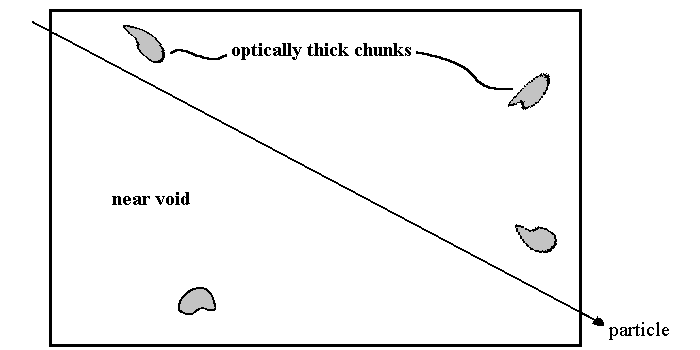
\includegraphics[height=6.45 cm,width= 12.9 cm]{nearvoid}
%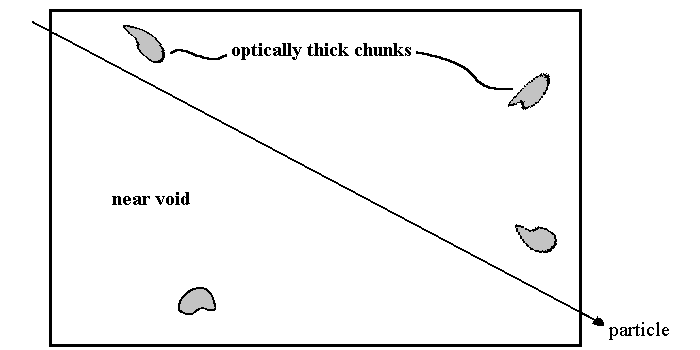
\includegraphics[height=6.45 cm,width= 12.9 cm]{nearvoid.jpg}
\caption{\footnotesize{Particle travelling through a near void with sparse chunks}}\label{fig_near_void}
\end{figure}
\n On the other hand, if we write the atomic mix description of $\textrm{Eqs.}\ ($\ref{exemploatmix}-\ref{ccexemploatmix}) neglecting the cross correlation term $\bl\tilde\Sigma_t\tilde\psi\bg$:
\begin{equation}
\frac{\partial\bl\psi\bg}{\partial u}+\bl\Sigma_t\bg\bl\psi\bg=0,
\end{equation}
\begin{equation}
\bl\psi(0)\bg = \bl\psi_s\bg,
\end{equation}
\n we will conclude that $\bl\psi\bg$ will be exponentially attenuated, with a scale length $1/\bl\Sigma_t\bg$, and it is clear that $\bl\Sigma_t\bg$ is very large, since $\Sigma_{t2}$ is very large.
Hence, this modeling will lead to essentialy no transmission through the system.
In general, neglecting the cross correlation term will underestimate particle transmission.

\section*{The Levermore-Pomraning Equations}

Following Adams, Larsen, and Pomraning \cite{adams_89} and Vasques et al. \cite{vasques_04}, let us assume a binary stochastic medium whose mixing statistics are arbitrary and known.
Also, for simplicity of exposition, we will consider only monoenergetic transport and isotropic scattering.
\begin{equation}\label{1.1}
\begin{split}
\frac{1}{v}\frac{\partial \psi}{\partial t}(\bm x,\bm\Omega,t) + \bm\Omega\cdot \bm\nabla
 \psi (\bm x,\bm\Omega,t) + &\Sigma_t(\bm x, t)\psi(\bm x,\bm\Omega,t) =
\\& = \frac{\Sigma_s(\bm x, t)}{4\pi}\int_{4\pi}\psi(\bm x,\bm\Omega',t)d\Omega' +
Q(\bm x,\bm \Omega, t).
\end{split}
\end{equation}

 If we introduce the characteristic functions
\begin{equation}\label{2.1}
\chi_i(\bm x) =
\Bigg\{
\begin{array}{l}
1, \;\;\textrm{if $\bm x$ is in material $i$}
\\ 0, \;\; \textrm{if $\bm x$ is in material $j\not=i$ }
\end{array},
\;\; i,j\in\{1,2\},
\end{equation}
the basic issue is that we do not know the functions $\chi_1(\bm x)$ and $\chi_2(\bm x)$, but we know that they satisfy
\begin{equation}\label{2.2}
\chi_1(\bm x)+\chi_2(\bm x) = 1.
\end{equation}
 (In the following discussion, the $\bm x$ and $t$ dependences are dropped for notational simplicity when convenient.)

 Multiplying Eq.$\,$(\ref{1.1}) by $\chi_i(\bm x)$, we can use
\begin{subequations}\label{2.3}
\begin{align}
\chi_i\big[\bm\Omega\cdot\bm\nabla\psi(\bm\Omega)\big] &= \bm\Omega\cdot\bm\nabla\chi_i\psi(\bm\Omega)-\psi(\bm\Omega)[\bm\Omega\cdot\bm\nabla\chi_i],
\\ \chi_i\Sigma_t &= \Sigma_{ti}\chi_i,
\\\chi_i\Sigma_s &= \Sigma_{si}\chi_i,
\\\chi_iQ(\bm\Omega) &= Q_i(\bm\Omega)\chi_i,
\end{align}
\end{subequations}
 to attain 
\begin{equation}\label{2.4}
\begin{split}
\frac{1}{v}\frac{\partial \chi_i\psi(\bm\Omega)}{\partial t}+\bm\Omega\cdot &\bm\nabla\chi_i\psi(\bm\Omega) + \Sigma_{ti}\chi_i\psi(\bm\Omega) =
 \\& =\frac{\Sigma_{si}}{4\pi}\int_{4\pi}\chi_i\psi(\bm\Omega')d\Omega'+Q_i(\bm\Omega)\chi_i +
 \psi(\bm\Omega)[\bm\Omega\cdot\bm\nabla\chi_i] .
 \end{split}
\end{equation}

 Defining $\bl \cdot \bg$ as the ensemble average operator over all statistical realizations, the probability of finding material $i$ at position $\bm x$ is given by
\begin{subequations}\label{2.5}
\begin{align}
 p_i = \bl\chi_i\bg,
\end{align}
and therefore we define
\begin{align}\label{2.5b}
\psi_i(\bm\Omega) = \frac{\bl\chi_i\psi(\bm\Omega)\bg}{\bl\chi_i\bg},
\end{align}
\end{subequations}
where $\psi_i$ is the ensemble average of $\psi(\bm x,\bm\Omega,t)$ over all physical realizations such that $\bm x$ is in material $i$.
By ensemble averaging Eq.$\,$(\ref{2.4}), we obtain 
\begin{equation}\label{2.6}
\begin{split}
\frac{1}{v}\frac{\partial [p_i\psi_i(\bm\Omega)]}{\partial t}+ \bm\Omega\cdot &\bm\nabla[p_i\psi_i(\bm\Omega)] + \Sigma_{ti}[p_i\psi_i(\bm\Omega)] =
\\& =
 \frac{\Sigma_{si}}{4\pi}\int_{4\pi}[p_i\psi_i(\bm\Omega')]d\Omega'+p_iQ_i(\bm\Omega) +
 \bl\psi(\bm\Omega)[\bm\Omega\cdot\bm\nabla\chi_i]\bg .
\end{split}
\end{equation}
 Further, from Eqs.$\,$(\ref{2.2}) and$\,$(\ref{2.5}) we deduce that
\begin{equation}\label{2.7}
\bl\psi(\bm\Omega)\bg = p_1\psi_1(\bm\Omega) + p_2\psi_2(\bm\Omega),
\end{equation}
which is the overall ensemble average of the angular flux.

To evaluate the term $\bl f_i(\bm x,\bm\Omega,t)\bg = \bl\psi(\bm x,\bm\Omega,t)[\bm\Omega\cdot\bm\nabla\chi_i(\bm x)]\bg$ on the right hand side of Eq.$\,$(\ref{2.6}), we consider the average value of $f_i(\bm x,\bm\Omega,t)$ over a volume $V$ and take the limit as $V$ approaches zero.
This yields
\begin{equation}\label{2.8}
\bl f_i(\bm x,\bm\Omega,t)\bg= 
\lim_{V \rightarrow 0} \bigg<\psi(\bm x,\bm\Omega,t)\bigg(\frac{1}{V}
\int_{V}\bm\Omega\cdot\bm\nabla\chi_i(\bm x)dV\bigg)\bigg>.
\end{equation}
 The ensemble average in Eq.$\,$(\ref{2.8}) is over all realizations.
 However, for a given realization, we have $\int_{V}\bm\Omega\cdot\bm\nabla\chi_i(\bm x)dV\not = 0$ only if there is an interface between materials $i$ and $j$ intersecting $V$.
 Therefore, we write
\begin{equation}
\bigg<\psi(\bm\Omega)\bigg(\frac{1}{V}
\int_{V}\bm\Omega\cdot\bm\nabla\chi_idV\bigg)\bigg> = 
P^* \bigg<\psi(\bm\Omega)\bigg(\frac{1}{V}
\int_{V}\bm\Omega\cdot\bm\nabla\chi_idV\bigg)\bigg>^*,
\end{equation}
 where $P^*$ is the probability that a realization has an interface that intersects $V$, and $\bl \cdot \bg^*$ is a restricted average defined to be an ensemble average over all realizations having an interface that intersects $V$.

Now, we consider $V$ to be a sphere of radius $\ep$ centered at position $\bm x$ at time $t$.
Assuming that there exists an interface intersecting this sphere, for $\ep$ small enough we can regard this interface as a plane with normal vector $\bm{n_i}$ pointing out of region $i$.
If we chose the $x$-axis perpendicular to this planar interface (as shown in Figure \ref{fig_1}),
\begin{figure}[t]
\centering
%\includegraphics[height=7 cm,width=8.75 cm]{local_coord_zaxis_2.ps}
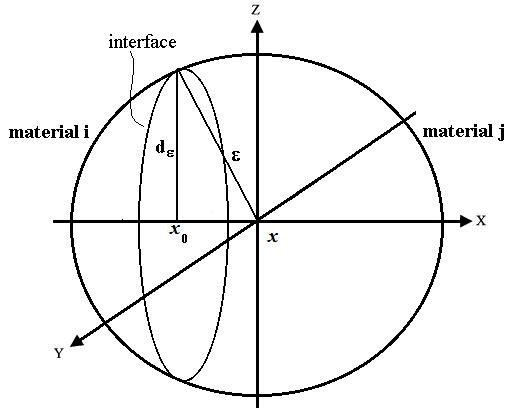
\includegraphics[height=7 cm,width=8.75 cm]{fig_1.jpeg}
\caption{Intersection of the interface with the sphere $V$}\label{fig_1}
\end{figure}
then the intersection of the interface with the sphere is a disc of radius $d_{\ep}=\sqrt{\ep^2-x_0^2}$ given by the intersection of the plane $x=x_0$ with the sphere, and $\bm{n_i} = \hat{\bm{e_x}}$.
In this coordinate system we have $\bm\nabla \chi(\bm x) = -\bm{n_i}\delta(x-x_0)$; thus
\begin{equation}
%\begin{split}
\frac{1}{V}\int_{V}\bm\Omega\cdot\bm\nabla\chi_i(\bm x)dV =
\frac{3}{4\pi\ep^3}\int_{V}[-\bm\Omega\cdot\bm{n_i}]\delta(x-x_0)dxdydz
%\\& = \frac{3}{4\pi\ep^3}[-\bm\Omega\cdot\bm{n_i}]\pi d_{\ep}^2
%\\&
 = \frac{3}{4\ep^3}[-\bm\Omega\cdot\bm{n_i}]d_{\ep}^2,
%\end{split}
\end{equation}
 and $\textrm{Eq.}\ ($\ref{2.8}) becomes
\begin{equation}\label{2.11}
\bl f_i(\bm x,\bm\Omega,t) \bg = \lim_{\ep\rightarrow 0}\bigg[-\frac{3}{4\ep^3}
P^*\bigg<[\bm\Omega\cdot\bm{n_i}]
\psi(\bm x,\bm\Omega,t)d_{\ep}^2\bigg>^*\bigg].
\end{equation}
 Let us define $\bl \cdot \bg^*_{\bm\Omega\cdot\bm{n_i}>0}$ to be the ensemble average over all realizations such that an interface intersects $V$ and $\bm\Omega$ points out of material $i$.
Then, since $\bm{n_i} = -\bm{n_j}$,
\begin{equation}
\begin{split}
\bigg<[\bm\Omega\cdot\bm{n_i}]
&\psi(\bm x,\bm\Omega,t) d_{\ep}^2 \bigg>^* =
\\& = \bigg<[\bm\Omega\cdot\bm{n_i}]
\psi(\bm x,\bm\Omega,t) d_{\ep}^2 \bigg>_{\bm\Omega\cdot\bm{n_i}>0}^*+
 \bigg<[\bm\Omega\cdot\bm{n_i}]
\psi(\bm x,\bm\Omega,t) d_{\ep}^2 \bigg>_{\bm\Omega\cdot\bm{n_i}<0}^*
\\& = \bigg<[\bm\Omega\cdot\bm{n_i}]
\psi(\bm x,\bm\Omega,t) d_{\ep}^2 \bigg>_{\bm\Omega\cdot\bm{n_i}>0}^*-
 \bigg<[\bm\Omega\cdot\bm{n_j}]
\psi(\bm x,\bm\Omega,t) d_{\ep}^2 \bigg>_{\bm\Omega\cdot\bm{n_j}>0}^*.
\end{split}
\end{equation}
Defining
\begin{subequations}
\begin{align}
\Psi_i^{\ep}(\bm x,\bm\Omega,t) &= \frac{\bl[\bm\Omega\cdot\bm{n_i}]\psi(\bm x,\bm\Omega,t)
d_{\ep}^2\bg^*_{\bm\Omega\cdot\bm{n_i}>0}}
{\bl[\bm\Omega\cdot\bm{n_i}]d_{\ep}^2\bg^*_{\bm\Omega\cdot\bm{n_i}>0}}
\end{align}
and
\begin{align}
\Psi_i(\bm x,\bm\Omega,t) &= \displaystyle{\lim_{\ep\rightarrow 0}}\Psi_i^{\ep}(\bm x,\bm\Omega,t),  
\end{align}
\end{subequations}
 we can rewrite Eq.$\,$(\ref{2.11}) as
\begin{equation}\label{2.14}
\begin{split}
\bl f_i (\bm\Omega) \bg &= \\&= \lim_{\epsilon\rightarrow 0}
\bigg[\frac{3}{4\ep^3}P^*\bigg(\Psi_j^\ep
\bl[\bm\Omega\cdot \bm{n_j}]d_{\ep}^2\bg^*_{\bm\Omega\cdot\bm{n_j}>0}
-\Psi_i^{\ep}\bl[\bm\Omega\cdot\bm{n_i}]d_{\ep}^2\bg^*_{\bm\Omega\cdot\bm{n_i}>0}\bigg)\bigg]
\\& = [\Psi_j(\bm\Omega) - \Psi_i(\bm\Omega)]\lim_{\epsilon\rightarrow 0}
\bigg[\frac{3}{4\ep^3}P^*\bl[\bm\Omega\cdot \bm{n_i}]d_{\ep}^2\bg^*_{\bm\Omega\cdot\bm{n_i}>0}\bigg],
\end{split}
\end{equation}
since the geometrical quantities $\bl [\bm\Omega\cdot\bm{n_i}]d_\ep^2 \bg^*_{\bm\Omega\cdot\bm{n_i}>0}$ are equal for $i\in\{1,2\}$.
We point out that Eq.$\,$(\ref{2.14}) is exact; in fact, with this choice of coordinates, the limit in the equation above is the same geometric quantity dependent upon the statistics that appears in \cite{adams_89} (we will see this next). 

We can now rewrite Eq.$\,$(\ref{2.6}) exactly as
\begin{equation}\label{lpquase}
\begin{split}
\frac{1}{v}\frac{\partial [p_i\psi_i(\bm\Omega)]}{\partial t}+ \bm\Omega\cdot &\bm\nabla[p_i\psi_i(\bm\Omega)] + \Sigma_{ti}[p_i\psi_i(\bm\Omega)] =
\\& \hspace{-1.0 cm} =
 \frac{\Sigma_{si}}{4\pi}\int_{4\pi}[p_i\psi_i(\bm\Omega')]d\Omega'+p_iQ_i(\bm\Omega) +
 \\& \hspace{1.0 cm}+
 [\Psi_j(\bm\Omega) - \Psi_i(\bm\Omega)]\lim_{\epsilon\rightarrow 0}
\bigg[\frac{3}{4\ep^3}P^*\bl[\bm\Omega\cdot \bm{n_i}]d_{\ep}^2\bg^*_{\bm\Omega\cdot\bm{n_i}>0}\bigg].
\end{split}
\end{equation}
Unfortunately, this result consists of two equations with four unknown functions, namely $\psi_1$, $\psi_2$, $\Psi_1$, and $\Psi_2$; thus, a closure is needed to make this formalism useful.
No simple exact relationship seems to exist relating $\psi_i$ (the ensemble average of $\psi$ over all physical realizations such that $\bm x$ is in material $i$ at time $t$) and $\Psi_i$ (the ensemble average of $\psi$ at interface points for which $\bm\Omega\cdot\bm{n_i}>0$).
Nevertheless, $\Psi_i$ can be approximated by simply equating it to $\psi_i$, in analogy with upwind differencing encountered in the numerical analysis of hyperbolic equations.
With this closure, one obtains the LP equations for arbitrary statistics as introduced in \cite{adams_89}.
It is important to point out that, in the case of time independent, purely absorbing Markovian media, equating $\Psi_i=\psi_i$ is not an approximation, but an exact identity.

Let us assume that the statistics of the medium is homogeneous.
In particular, we assume that
\begin{tabbing}
\hspace{0.8 cm}{\textrm 1)} the points $x_0$ in the Figure \ref{fig_1} are uniformly\\ \hspace{1.23 cm}distributed on
$-\ep<x_0<\ep$;
\\
\hspace{0.8 cm}{\textrm 2)} the normal vectors of interfaces passing through $V$ are uniformly distributed on the \\ \hspace{1.23 cm}unit sphere.
\end{tabbing}
 Then, using $\bm\Omega\cdot\bm{n_i} = \mu$ and $d_\ep^2 = \ep^2-x_0^2$, we obtain
\begin{equation}
\begin{split}
\bl(\bm\Omega\cdot\bm{n_i})d_\ep^2\bg^*_{\bm\Omega\cdot\bm{n_i}>0} &=
\bl \mu(\ep^2-x_0^2)\bg^*_{\mu>0} 
\\&
=\int_0^1\bigg(\frac{1}{2\ep}\int_{-\ep}^\ep \mu(\ep^2-x_0^2)dx_0\bigg)d\mu 
%\\& =
%\frac{1}{2}\bigg(\frac{1}{2\ep}\frac{4\ep^3}{3}\bigg)
\\& =
\frac{\ep^2}{3}.
\end{split}
\end{equation}
 Introducing this result into Eq.$\,$(\ref{2.14}), we get
\begin{equation}\label{3.2}
\bl f_i (\bm\Omega) \bg
% = [\Psi_j(\bm\Omega)-\Psi_i(\bm\Omega)]\lim_{\epsilon\rightarrow 0}
%\bigg[\frac{3}{4\ep^3}\frac{\ep^2}{3}P^*\bigg]
= [\Psi_j(\bm\Omega)-\Psi_i(\bm\Omega)]\lim_{\epsilon\rightarrow 0}
\bigg[\frac{1}{4\ep}P^*\bigg].
\end{equation}
\begin{figure}[h]
\centering
%\includegraphics[height=2.5 cm,width=10 cm]{perpendic_interf.ps}
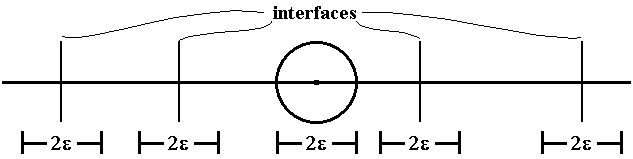
\includegraphics[height=2.5 cm,width=10 cm]{fig_2.jpg}
\caption{Arbitrary infinite line intersecting interfaces perpendicularly}\label{fig_2}
\end{figure}

 It is also possible to approximate $P^*$.
 To do this, let us consider an arbitrary infinite line through the point $\bm x$, and let us assume it to be the travel path of the particle in the system.
 Then, it can be seen from Figure \ref{fig_2} that an interface intersects the pathline within $V$ only if the point $\bm x$ lies within a distance $\ep$ of an interface.
This creates a line segment of width $2\ep$ about each interface, such that if $\bm x$ is in one of these segments, then an interface intersects the pathline within $V$.
 Over a very large length of this line, spanning $m$ chunks of material $1$ and $m$ chunks of material $2$ (with $m\rightarrow\infty$), we have
\begin{subequations}\label{3.3}
\begin{align}
(2m)(2\ep) &= 4m\ep \nonumber
\\& = \left(
\begin{matrix}
\textrm{the length of the line segments such that if $\bm x$ lies on}
\\ \textrm{one of these segments, then an interface intersects $V$}
\end{matrix}
\right)
\end{align}
 and
\begin{align}
m(\Lambda_1 + \Lambda_2) = (\textrm{total length of the line}),
\end{align}
\end{subequations}
where $\Lambda_i$ is the mean chord length in material $i$. 
The ratio of these equations is $P^*$.
That is,
\begin{equation}\label{3.4}
P^* = \frac{4\ep}{\Lambda_1 + \Lambda_2}.
\end{equation}
 One can easily see that this expression has the right qualitative behavior.
 It correctly limits to zero as $\ep \rightarrow 0$, and as $\Lambda_1,\Lambda_2\rightarrow \infty$.
 Introducing Eq.$\,$(\ref{3.4}) into Eq.$\,$(\ref{3.2}), we obtain
\begin{equation}\label{3.5}
\bl f_i (\bm\Omega) \bg =
[\Psi_j(\bm\Omega)-\Psi_i(\bm\Omega)]\lim_{\epsilon\rightarrow 0}
\bigg[\frac{1}{4\ep}\bigg(\frac{4\ep}{\Lambda_1+\Lambda_2}\bigg)\bigg]=
\frac{\Psi_j(\bm\Omega)-\Psi_i(\bm\Omega)}{\Lambda_1+\Lambda_2}.
\end{equation}

For binary homogeneous statistics, the following identity holds:
\begin{equation}\label{3.6}
p_i = \frac{\Lambda_i}{\Lambda_1+\Lambda_2},\;\; i\in\{1,2\};
\end{equation}
it follows that
\begin{equation}\label{3.7}
\bl f_i (\bm\Omega) \bg = \frac{p_j\Psi_j(\bm\Omega)}{\Lambda_j}
-\frac{p_i\Psi_i(\bm\Omega)}{\Lambda_i}.
\end{equation}
Equating $\Psi_i = \psi_i$, this result is the classic LP expression for the coupling term in Markovian homogeneous statistics.
The LP expression is then written as 
\begin{equation}%\label{eq_averaged_1}
\begin{split}
\frac{1}{v}\frac{\partial (p_i\psi_i)}{\partial t}+ \bm\Omega\cdot &\nabla(p_i\psi_i) + \Sigma_{ti}(p_i\psi_i) =
\\& =
 \frac{\Sigma_{si}}{4\pi}\int_{4\pi} p_i\psi_i(\bm x,\bm\Omega',t)d\Omega'+p_iQ_i +
 \frac{p_j\psi_j}{\Lambda_j} -  \frac{p_i\psi_i}{\Lambda_i},
\end{split}
\end{equation}
and the general case (general scattering, energy dependent) is straightforwardly given by
\begin{equation}\label{eq_averaged_closed}
\begin{split}
\frac{1}{v}&\frac{\partial (p_i\psi_i)}{\partial t}+ \bm\Omega\cdot \nabla(p_i\psi_i) + \Sigma_{ti}(E)(p_i\psi_i) =
\\& =
 \int_0^{\infty}\int_{4\pi} \Sigma_{si}(E\rightarrow E',\bm\Omega\cdot\bm\Omega')p_i\psi_i(\bm x,E',\bm\Omega',t)d\Omega'dE'+p_iQ_i +
 \frac{p_j\psi_j}{\Lambda_j} -  \frac{p_i\psi_i}{\Lambda_i},
\end{split}
\end{equation}

In order to extend these considerations to nonstatic physical realizations of the mixing, we define
\begin{equation}
\chi_i(\bm x,t) =
\Bigg\{
\begin{array}{l}
1, \;\;\textrm{if $\bm x$ is in material $i$ at time $t$}
\\ 0, \;\; \textrm{if $\bm x$ is in material $j\not=i$ at time $t$}
\end{array}.
\end{equation}
Applying the same procedure as before, a new term will appear, given by $(h_i)$ in
\begin{equation}
\begin{split}
\frac{1}{v}\bigg(\chi_i\frac{\partial \psi}{\partial t}\bigg) =
\frac{1}{v}\frac{\partial (\chi_i\psi)}{\partial t}\;\;\; -\;\;\;
&\underbrace{\frac{1}{v}\bigg(\psi\frac{\partial \chi_i}{\partial t}\bigg)}.
\\& \hspace{0.7 cm}(h_i)
\end{split}
\end{equation}
We define $p_i(\bm x,t)$, the probability of finding material $i$ at point $\bm x$ and time $t$, by
\begin{equation}
p_i(\bm x,t) = \bl \chi_i(\bm x,t) \bg ,
\end{equation}
and the ensemble-averaged angular flux over all physical realizations such that $\bm x$
is in material $i$ at time $t$ by
\begin{equation}
\psi_i(\bm x,E,\bm\Omega,t) = \frac{\bl \chi_i(\bm x,t)\psi(\bm x,E,\bm\Omega,t) \bg}{\bl \chi_i(\bm x,t) \bg}.
\end{equation}
Treating $\bl h_i \bg$ in analogy with the way we treated $\bl f_i \bg$, we find
\begin{equation}\label{eq_spat_time}
\begin{split}
\frac{1}{v}\frac{\partial (p_i\psi_i)}{\partial t}&+  \bm\Omega\cdot\nabla(p_i\psi_i) +
\Sigma_{ti}(p_i\psi_i) =
\\& \int_0^{\infty}\int_{4\pi} \Sigma_{si}(E\rightarrow E',\bm\Omega\cdot\bm\Omega')p_i\psi_i(\bm x,E',\bm\Omega',t)d\Omega'dE' +
 \\& \hspace{1.5cm}+p_iQ_i +
\bigg(\frac{p_j\Psi_j}{\Lambda_j} -  \frac{p_i\Psi_i}{\Lambda_i}\bigg)+
\bigg(\frac{p_j\hat\Psi_j}{\hat\lambda_j} -  \frac{p_i\hat\Psi_i}{\hat\lambda_i}\bigg),
\end{split}
\end{equation}
where
\begin{equation}\label{lambda_chapeu}
\frac{p_i(\bm x,t)}{\hat\lambda_i(\bm x,t)}=\frac{1}{v}\lim_{T\rightarrow 0}
\bigg[\frac{1}{T}\bl N_i \bg\bigg]
\end{equation}
\n and
\begin{equation}\label{psi_chapeu}
\hat\Psi_i = \bl \psi \bg^{\ddagger}_{i\rightarrow j}.
\end{equation}
\n In $\textrm{Eq.}\ ($\ref{lambda_chapeu}), $T$ is a time interval and $N_i$ is the number of transitions from material $i$ to material $j\not= i$ in $T$ at space point $\bm x$.
In $\textrm{Eq.}\ ($\ref{psi_chapeu}), the operator $\bl\cdot\bg^{\ddagger}_{i\rightarrow j}$ is a restricted average, defined to be an ensemble average over realizations that undergo a transition from material $i$ to material $j$ at a given space point $\bm x$ at a time $t$.

Again, a simple closure is obtained by setting $\Psi_i = \hat\Psi_i=\psi_i$.
Also, we can define a composite coupling coefficient $\tilde\lambda_i$ according to
\begin{equation}
\frac{1}{\tilde\lambda_i} = \frac{1}{\Lambda_i} + \frac{1}{\hat\lambda_i},
\end{equation}
\n and applying these arguments in $\textrm{Eq.}\ ($\ref{eq_spat_time}), it becomes identical to $\textrm{Eq.}\ ($\ref{eq_averaged_closed}) (with the terms $\Lambda_i$ replaced by $\tilde\lambda_i$). 

 \setlength{\baselineskip}{12pt}
\begin{thebibliography}{300}

\bibitem{dumas_00} D{\footnotesize UMAS}, L. {\footnotesize AND} G{\footnotesize OLSE}, F.
``Homogenization of Transport Equations",
\textit{SIAM J. Appl. Math.} {\bf 60} (2000), 1447. %1470

\bibitem{larsen_03} L{\footnotesize ARSEN}, E. W. ``Asymptotic Derivation of the Atomic Mix Diffusion
Model for 1-D Random Media",
\textit{Trans. Am. Nucl. Soc.} %Transactions of the American Nuclear Society
{\bf 89} (2003), 296. %297

\bibitem{larsen_rio} L{\footnotesize ARSEN}, E. W., V{\footnotesize ASQUES}, R., {\footnotesize AND} V{\footnotesize ILHENA}, M. T. ``Particle Transport in the 1-D Diffusive Atomic Mix Limit", in
\textit{Mathematics and Computation, Supercomputing, Reactor Physics and Nuclear and Biological Applications.} Avignon, France (2005), in CD-ROM.

\bibitem{adams_89} A{\footnotesize DAMS}, M. L., L{\footnotesize ARSEN}, E. W.,
{\footnotesize AND}
P{\footnotesize OMRANING}, G. C.
``Benchmark Results for Particle Transport in a Binary Markov Statistical Medium",
\textit{J. Quant. Spectrosc. Radiat. Transfer} {\bf 42} (1989), 253.%266
 
 \bibitem{vasques_04} V{\footnotesize ASQUES}, R., V{\footnotesize ILHENA}, M. T.,
T{\footnotesize HOMPSON}, M., {\footnotesize AND} L{\footnotesize ARSEN}, E. W.
``State of Art of Particle Transport Theory in Stochastic Media",
in
\textit{Proc. XXV Iberian Latin American Congress on Computational Methods in Engineering},
Recife (2004), on CD-ROM.%211 V. C. Boffi et al., eds.,


\end{thebibliography}


\end{document}
Contact GitHub 